% !TEX program = xelatex
\documentclass[11pt,fontset=fandol]{ctexart}

\usepackage[a4paper,margin=2.0cm]{geometry}
\usepackage{booktabs}
\usepackage{tabularx}
\usepackage{array}
\usepackage{xcolor}
\usepackage{hyperref}
\usepackage{longtable}
\usepackage{graphicx}

\definecolor{linkblue}{HTML}{2F6FAB}
\definecolor{muted}{HTML}{5D6D7E}
\definecolor{softgray}{HTML}{F4F6F7}
\definecolor{softred}{HTML}{B03A2E}
\definecolor{softgreen}{HTML}{1E8449}

\hypersetup{
  colorlinks=true,
  linkcolor=linkblue,
  urlcolor=linkblue
}

\setlength{\parindent}{0pt}
\setlength{\parskip}{0.55em}
\emergencystretch=3em
\renewcommand{\arraystretch}{1.22}
\newcolumntype{Y}{>{\raggedright\arraybackslash}X}
\newcolumntype{L}[1]{>{\raggedright\arraybackslash}p{#1}}
\newcommand{\code}[1]{\texttt{\detokenize{#1}}}
\newcommand{\good}[1]{\textcolor{softgreen}{#1}}
\newcommand{\bad}[1]{\textcolor{softred}{#1}}
\urlstyle{same}

\title{\bfseries OpenCollab SWE-bench 做题 Harness 与 V1/V2 对比阶段报告}
\author{Kai / Codex}
\date{2026-07-03}

\begin{document}
\sloppy
\maketitle

\section{摘要}

本次工作围绕 OpenCollab 在 SWE-bench 上的 V1/V2 对比展开。早期 V2 结果显示 11 题中已有 10 个有效 patch 完成官方评测，结果为 \bad{0 resolved / 10 unresolved}。直接把这个结果解释为 V2 架构失败会混入基础设施问题，因为若干题的结构化 agent 阶段出现 Connection error、空 patch 或 workflow incomplete。后续工作把连接失败、schema 失败、semantic blocker 和官方评测失败拆开记录，并把生成 patch 与评测 patch 合并为一个可维护的“做题”过程。

当前最重要的事实有四个。第一，11 题 V2 中有 7 题属于完整 workflow 且有 patch，1 题有 patch 但 workflow incomplete，3 题是 infra invalid；这些分类决定了后续科研比较时哪些样本可以进入 V1/V2 架构分析。第二，\bad{0 resolved / 10 unresolved} 这个差结果很有研究价值，它暴露了技术失败伪装成语义失败、验证阶段同质化、自动评测缺口、费用统计混账和墙钟时间低估等一组问题。第三，V1 已通过的两道题在 V2 final harness 下结果分化：\code{django__django-14730} 仍然通过，\code{django__django-11019} 未通过。第四，自动做题脚本 \code{scripts/swe_auto_eval_driver.py} 已经能够发现非空 patch、启动远端 official eval、识别 report、刷新 Markdown/JSON 状态，并处理 stale tmux、SSH 断连和 dataset 单对象等实际问题。

\section{文档与目录约定}

组会文档统一放在 \code{docs/group_meetings/} 下，每次组会使用一个带日期和主题的子目录。本次目录为：

\code{docs/group_meetings/2026-07-03-swebench-v2-harness/}

目录内保存本文的 LaTeX 源文件和编译后的 PDF。后续每次组会复用这一组织方式，把实验状态、关键表格、证据路径和下一轮计划写成可直接发送或展示的 PDF。

\section{V2 十一题实验状态}

V2 11 题的监控看板来自 \code{docs/monitoring/swe_v2_11_status.md} 和 \code{docs/monitoring/swe_v2_11_status.json}。最后一次刷新显示，原始结果行共 11 条，当前没有远端 tmux 运行。完整 workflow 且有 patch 的样本为 7 个，有 patch 但 workflow incomplete 的样本为 1 个，infra invalid 为 3 个，空 patch invalid 为 0 个。官方评测中已有 10 个 report，resolved 为 0，unresolved 为 10。

\begin{table}[h]
\centering
\begin{tabularx}{0.92\linewidth}{L{5.4cm}rY}
\toprule
指标 & 数值 & 说明 \\
\midrule
总题数 & 11 & 本轮 V2 目标样本 \\
完整 workflow 且有 patch & 7 & 可进入 V2 完整运行分析 \\
patch 但 workflow incomplete & 1 & 可做诊断，科研比较需单列 \\
infra invalid & 3 & 连接或基础设施污染，不能计入语义失败 \\
空 patch invalid & 0 & 当前看板中已无空 patch invalid \\
官方评测 report & 10 & 已完成 official eval 的 patch 数 \\
官方 resolved / unresolved & 0 / 10 & 已评测 patch 全部未通过 \\
平均单题模型运行耗时 & 21.9 min & 来自 workflow active duration \\
累计 workflow token & 15,581,955 & metrics total，含一个估算缺口 \\
估算费用 & \$10.22 & 轨迹账本加缺口估算 \\
\bottomrule
\end{tabularx}
\end{table}

这个表的核心作用是把结果分层。Infra invalid 样本包括 \code{astropy__astropy-7746}、\code{django__django-11905} 和 \code{django__django-14155}。这些题的失败不能作为 V2 语义能力证据。另一个特殊样本 \code{django__django-11283} 有 patch 且官方评测 unresolved，但 workflow incomplete，因此可以用于诊断，不能和完整 V2 正常完成样本混在一起比较。

\section{差结果暴露出的发现}

V2 这轮效果很差，这本身是一个值得研究的现象。单句判定 V2 思路成败没有太多信息量；真正有价值的是，失败把系统里原先混在一起的几类问题强行分离出来。早期看起来只是“10 个 patch 全部未通过”，继续追踪后可以看到，里面同时存在基础设施错误、workflow 状态表达不足、验证阶段探针不足、官方评测自动化不足、成本统计边界不清和时间估计偏差。每一类问题都对应一条可以修的 Harness 设计原则。

第一个发现是 transport failure 会伪装成 semantic failure。结构化 agent 在 Connection error、API timeout、代理不可达或反向隧道断开时返回空结果，旧流程会把空结果转成默认 blocker 或 verifier fail。这样一来，外层看到的是 workflow incomplete 或 final verifier 不通过，实际原因却是某个结构化阶段没有拿到模型输出。这个发现解释了 \code{astropy__astropy-7746}、\code{django__django-11905}、\code{django__django-14155} 等样本为什么不能进入 V1/V2 架构比较。

第二个发现是“生成了 patch”这个事件不够完整。一个样本可能有非空 patch，但 workflow 没有正常完成；也可能 workflow 完成，但 official eval 未跑；还可能 official eval 已经跑完，但 report 路径没有被脚本发现。旧流程里这些状态容易被压缩成“做完”或“失败”，导致监控和科研结论都变粗。后续把状态拆成 \code{patch_done_and_workflow_done}、\code{patch_done_but_workflow_incomplete}、\code{infra_invalid}、\code{empty_patch_invalid}、\code{official_resolved} 和 \code{official_unresolved}，这个拆分直接改变了后续实验的统计边界。

第三个发现是 V2 的多个验证角色可能重复验证同一组弱证据。在 \code{django__django-11019} 中，V2 的 patch 能通过 issue repro 和局部测试，却漏掉稳定交错顺序这一核心语义。更具体地说，多个阶段接受了 \code{Media.merge([1,2],[3,2])} 这一类已经接近 issue 文本的例子，但没有构造 \code{Media.merge([1,2],[3,4]) == [1,3,2,4]} 这样的判别性探针，也没有主动搜索 Django 内已有的 \code{stable_topological_sort()}。这说明增加评审角色本身不会自动带来验证多样性；Harness 必须要求判别性 probe、现有工具审查和 API/warning 兼容检查。

第四个发现是自动评测本身也需要成为 Harness 的一部分。刚开始 patch 生成与官方评测是分开的，需要人工发现非空 patch、手动组装 predictions、手动启动 official eval，再手动从不同目录找 report。实际运行中出现过 tmux 已退出但状态仍显示 active、官方 report 写在 side-car 目录却被误判为 missing report、SSH 短暂断连导致 watch 停止、dataset 单对象 JSON 需要包装成 list 等问题。这些问题不属于模型能力，却会直接污染“做题是否完成”的判断。

第五个发现是成本和时间需要分账。代理账本、远端轨迹账本、workflow metrics 各自代表不同层级，不能相加。墙钟时间也不能简单等同于模型 active 时间，因为其中包含等待、接续、镜像准备、重跑和人工检查空档。看板后来同时展示 active workflow time、wall span、overhead、trajectory usage 和 proxy usage，才让“为什么跑得这么慢、到底花了多少钱”变成可以解释的问题。

\begin{table}[h]
\centering
\begin{tabularx}{0.96\linewidth}{L{3.7cm}Y Y}
\toprule
发现 & 现象 & 对应修复 \\
\midrule
transport 伪装成语义失败 & Connection error 后结构化 verdict 为空，被外层当成 blocker 或 verifier fail & stage-level retry，错误分类为 transport / infra invalid，metrics 记录 error count \\
patch 状态过粗 & 非空 patch、workflow done、official eval done 被混在一起 & 看板增加分层状态，official eval 结果单独记录 \\
验证同质化 & 多个验证角色重复 issue repro，缺少推翻错误算法的 probe & final verifier coverage 要求判别性 probe、repo-native helper audit、API compatibility checks \\
评测自动化缺口 & 需要人工启动 official eval，report 路径和 tmux 状态容易误判 & 新增 \code{scripts/swe_auto_eval_driver.py}，自动发现 patch、启动 eval、刷新状态 \\
成本与时间混账 & 代理账、轨迹账、metrics total 与墙钟时间混用 & 看板拆分 token 来源、费用估算、active time 和 overhead \\
\bottomrule
\end{tabularx}
\end{table}

因此，V2 的差结果带来的主要发现是：委员会式结构的风险不只在“模型会写错代码”，还在“验证角色会形成同质化判断”“技术错误会污染语义统计”“做题状态会被粗粒度脚本掩盖”。这轮修复的价值就在于把这些风险变成可观测、可重试、可排除、可对比的实验变量。

\section{V1 已通过两题的 V2 补测}

V1 报告中有两道已通过题：\code{django__django-11019} 和 \code{django__django-14730}。对这两题使用加厚后的 V2 final harness 重新生成 patch 并做官方评测后，结果分化明显。

\begin{table}[h]
\centering
\begin{tabularx}{0.92\linewidth}{L{4.2cm}cccY}
\toprule
题目 & V1 & V2 final harness & V2 F2P/P2P & 解释 \\
\midrule
\code{django__django-11019} & resolved & unresolved & 13 / 0 & V2 patch 可 apply，无 infra/schema/rate-limit 错误，但语义上没有满足稳定交错排序要求 \\
\code{django__django-14730} & resolved & resolved & 0 / 0 & V2 final harness 保住了这个 V1 已通过样本 \\
\bottomrule
\end{tabularx}
\end{table}

\code{django__django-11019} 的差异已经整理在 \code{docs/monitoring/swe_v2_11019_v1_v2_regression_analysis.md}。V1 使用 Django 已有的 \code{stable_topological_sort()}，V2 手写拓扑排序。V2 的贪心规则能通过 issue 文本中的局部例子，却没有满足更一般的稳定交错顺序。例如 \code{Media.merge([1, 2], [3, 4])} 的官方期望是 \code{[1, 3, 2, 4]}，V2 输出会退化为 \code{[1, 2, 3, 4]}。这说明 V2 的后半段评审没有形成足够强的判别性探针。

\section{Harness 加厚内容}

这轮修复重点是把技术失败和语义失败分开。结构化 agent 的连接错误、API timeout、代理不可达、反向隧道断开等情况现在应归为 transport 或 infra failure；schema capture、schema validation、semantic blocker 也需要拆开统计。这样可以避免把 Connection error 伪装成 final verifier 的语义拒绝。

V2 workflow 和 runtime 的加厚覆盖了结构化 agent stage-level retry、错误分类、metrics 记录和 workflow 状态记录。相关改动集中在 \path{opencollab/opencollab/application/workflow.py}、\path{opencollab/opencollab/application/structured_output.py}、\path{opencollab/opencollab/bootstrap/workflow_runtime.py}、\path{workflows/swe_committee_v2.py}、\path{swebench/gen_prediction_workflow.py} 以及对应测试。新增或更新的测试覆盖 workflow runtime、structured output、SWE committee V2、生成预测 workflow 和 evaluator workflow。

V2 final verifier 现在需要写出 \code{verification_coverage}，其中包含判别性 probe、repo-native helper reuse audit 和 API compatibility checks。对于 \code{django__django-11019} 这类图算法样本，final verifier 必须解释是否复用仓库已有工具，并给出能区分错误手写算法与正确实现的探针。若 coverage 缺失，\code{workflows/swe_committee_v2.py} 中的 coverage blocker 会把 final PASS 转成 \code{CONCRETE_BLOCKER}，从而触发下一轮修复。

\begin{table}[h]
\centering
\begin{tabularx}{0.96\linewidth}{L{4.2cm}Y}
\toprule
问题类型 & 当前处理方式 \\
\midrule
transport / connection failure & stage-level retry，重试耗尽后标记 infra invalid，保留日志和 patch \\
schema capture / validation failure & 独立计数，避免落入普通 semantic blocker \\
workflow incomplete & 与 patch done 分开展示，official eval 可用于诊断 \\
official unresolved & 只有官方 report 显示 tests fail 时才进入语义分析 \\
empty patch & 单独标记，先检查真实模型输出和 staged diff 来源 \\
\bottomrule
\end{tabularx}
\end{table}

下面把这轮真正遇到过的 Harness 问题展开成几个修复案例。这样看起来会比“加了重试和分类”更直观：每个案例都包含坏现象、它怎样污染实验、以及代码里如何处理。

\subsection{案例一：Connection error 被误判成语义拒绝}

最早暴露的问题出现在结构化 agent 阶段。V2 workflow 里大量关键节点使用 \code{ctx.agent(..., schema=..., label=...)} 产出结构化 verdict，例如 \code{final-verifier:r1}、\code{post-validation-factory:r1}、\code{existing-tests-approved-validation:r1}。旧实现里，一旦模型连接失败或代理连接断开，\code{_run_structured_agent()} 会捕获异常并返回 \code{None}。外层 workflow 无法区分“模型没有返回”和“模型返回了失败 verdict”，于是会生成默认 blocker，例如“Final verifier returned no structured verdict.”。这会把网络错误写成语义失败。

这个问题在 \code{astropy__astropy-7746}、\code{django__django-11905}、\code{django__django-14155} 上很明显。轨迹里可以看到 \code{structured agent failed (...): Connection error.}，随后 workflow 用完三轮，状态变成 incomplete。若直接把这些样本计入 V2 失败，就会把代理或反向隧道故障算成委员会设计失败。

修复方式分两层。第一层在 \code{opencollab/opencollab/application/workflow.py} 中加入结构化阶段原地重试：\code{STRUCTURED_TRANSPORT_RETRY_DELAYS = (10.0, 30.0, 90.0)}，也就是同一个 label 先等 10 秒，再等 30 秒，再等 90 秒。重试期间会写入 \code{workflow_failure_classification}，记录 \code{transport_error}、stage、label、attempt 和 max attempts。第二层是在重试耗尽后抛出 \code{WorkflowInfraError}，由 \code{workflow_runtime.py} 和 evaluator 把整题标为 \code{infra_invalid}，并把 \code{transport_error_count}、\code{rate_limit_error_count}、\code{schema_failure_count} 写入 metrics。这样，Connection error 只能进入基础设施失败分类，不能变成 \code{CONCRETE_BLOCKER} 或 \code{FAIL_WITH_EVIDENCE}。

\begin{table}[h]
\centering
\begin{tabularx}{0.96\linewidth}{L{3.2cm}Y Y}
\toprule
旧行为 & 污染方式 & 新行为 \\
\midrule
\code{Connection error} 后返回 \code{None} & 外层生成默认 verifier fail，三轮后 incomplete & 同一 label 重试 10/30/90 秒，耗尽后 \code{infra_invalid} \\
schema 阶段异常没有分类 & 看板无法区分网络、schema 和语义 blocker & metrics 记录 \code{transport/rate-limit/schema} 计数 \\
incomplete 样本进入总体失败统计 & V2 架构比较被基础设施污染 & 看板单列 \code{infra_invalid} 与 \code{patch_done_but_workflow_incomplete} \\
\bottomrule
\end{tabularx}
\end{table}

\subsection{案例二：结构化输出失败被压成空 verdict}

另一个更隐蔽的问题是 schema capture failure。结构化 agent 有时会生成自然语言解释，却没有调用 \code{structured_output} 工具；也有可能调用工具但字段缺失，不能满足 schema。旧流程把这些情况也压成 \code{None}，和连接失败、模型拒绝、真实语义 blocker 混在一起。

修复后，schema 捕获和 schema 校验各自有独立分类。\code{workflow.py} 增加 \code{schema_capture_failure_count}、\code{schema_validation_failure_count} 和总的 \code{schema_failure_count}。结构化 prompt 末尾统一追加“必须调用 \code{structured_output} 工具”的指令；若第一次 session 没有有效 payload，会开启一次强制提交式的 corrective retry，提示模型基于已有信息立刻提交结构化结果。这个 retry 使用命名 tool choice 指向 \code{structured_output}，端点拒绝强制 tool choice 时再降级为 auto。这样做的意义是：schema 层问题会被当成结构化通信问题处理，语义状态机只消费真实结构化 verdict。

这个修复对 V2/V3 都重要。委员会模式的每个节点都依赖 JSON verdict 传递状态。如果一个节点没有结构化输出，后续节点读到的是“缺失消息”，语义上等同于通信断点。以前缺失消息会被解释成反对意见；现在缺失消息会先被重试和分类。

\subsection{案例三：任务快到墙钟上限时已经找到改法却没写出 patch}

做题过程中还出现过另一种时间问题：模型已经定位到修改点，但接近单题硬超时时仍在解释、验证或搜索，最后没有把补丁写入工作区。对外看起来是空 patch 或无效 patch，实际是时间管理失败。

\code{workflow.py} 加了 \code{DEFAULT_DEADLINE_MARGIN_SECONDS = 120.0}。当 workflow 发现距离硬上限只剩约 120 秒时，\code{ctx.time_low()} 会触发保守路径，让 workflow 尽快进入最终写入或结果保存。这个改动的目的很具体：把“已经知道该改哪里”转成落盘 patch，而不是让单题死在最后几分钟。对于 SWE-bench 来说，晚一点的验证可以交给 official eval，空 patch 没有诊断价值。

\subsection{案例四：生成 patch 和 official eval 分离导致人工盯跑}

早期流程把“生成 patch”和“评测 patch”分成两件事。生成端写完 \code{predictions.jsonl} 后，需要人工检查是否非空、手动拼 official eval 输入、手动开 tmux、手动找 report。这在小样本时还能勉强维护，一旦同时跑 V2 11 题、V1 solved 两题、V3 经典两题，就会出现空档和重复判断。

\code{scripts/swe_auto_eval_driver.py} 解决的是这个具体问题。它从远端 \code{predictions.jsonl} 发现非空 patch，按 \code{instance id + patch sha} 生成候选，创建 side-car 输入文件，启动 official eval tmux，然后把状态写到远端 \code{status.json/status.md} 与本地 \code{docs/monitoring/swe_auto_eval_status.json/md}。它还会识别 active generation session，避免 patch 还在生成时抢先评测。

这个脚本也修了几个真实边界。第一，tmux 已经退出但状态文件还写着 active 时，脚本会用 tmux 当前状态重新解释。第二，official eval report 有时在 side-car 根目录，有时在 \code{official_eval/logs/run_evaluation/...}，脚本会多路径查找。第三，dataset 有时是单对象 JSON，官方评测需要 list，脚本会规范成单元素 list 并校验 \code{instance_id}。第四，SSH 短暂断连时，脚本写 \code{ssh_error} 快照，watch 模式下一轮继续。第五，side-car 带锁，减少两个监控进程重复启动同一个 patch。

\begin{table}[h]
\centering
\begin{tabularx}{0.96\linewidth}{L{4.0cm}Y}
\toprule
脚本边界 & 修复方式 \\
\midrule
tmux 已退出但旧状态仍 active & 以当前 tmux session 与 report 文件重新计算状态 \\
report 路径漂移 & 同时搜索 side-car 根目录、official eval 日志目录和常见输出目录 \\
dataset 是单对象 JSON & 自动包装成 list，校验 instance id \\
SSH 短暂断开 & 写入 \code{ssh_error}，watch 下一轮继续 \\
重复启动同一候选 & side-car lock 与 patch sha 候选 id \\
生成未结束就评测 & 检测 \code{swe_v2_} 和 \code{swe_v3_} 生成会话 \\
\bottomrule
\end{tabularx}
\end{table}

\subsection{案例五：V3 早期观察阶段被旧 solver prompt 带偏}

V3 第一次跑经典两题时暴露了一个新 Harness 问题：V3 的早期委员会本来只应该读代码、盘点事实、审查已有工具和生成候选契约，但它们继承了旧 SWE-bench agent prompt 中“必须编辑源码”的强指令。这会让只读阶段也倾向于寻找编辑动作，导致工具调用和 token 消耗异常，甚至干扰后续契约生成。

修复放在 \code{swebench/gen_prediction_workflow.py}。现在 \code{swe-committee-v3} 有独立的 \code{V3_WORKFLOW_AGENT_PROMPT}，里面明确说明角色和权限由 workflow label 决定：只有 file-write/apply-patch 类型的求解阶段可以改代码；语义盘点、工具审查、候选契约、探针和最终裁决阶段都只能读、分析和结构化输出。这个改动让 V3 的“先观察，再假设，再裁决”有了系统提示层面的保障。

\subsection{案例六：V3 会话没有被 preflight 和 auto eval 识别}

把 V3 接入现有做题脚本时还出现了一个命名边界。早期 \code{swe_v2_preflight.py} 和 \code{swe_auto_eval_driver.py} 只识别 \code{swe_v2_} 开头的生成 tmux。V3 会话名是 \code{swe_v3_django_11019} 或 \code{swe_v3_django_15252}。这会导致两个风险：preflight 可能漏报已有 V3 正在生成，auto eval 也可能在 V3 patch 还没写完时启动官方评测。

修复很小，但很关键。两个脚本都把 active generation session 的检测改为同时接受 \code{swe_v2_} 和 \code{swe_v3_}，并排除 \code{official_eval} 会话。修完后，用 V3 活跃会话做 dry-run，脚本会明确报告 \code{active_generation_sessions: ["swe_v3_django_11019"]}，并且不会启动 official eval。这个例子说明 Harness 加厚不一定都是大改，有些是把命名约定从 V2 专用提升为多版本通用。

\section{委员会 V3 设计}

V3 的基本判断是：契约思想仍然有价值，但契约裁决权必须后置。V2 在 \code{django__django-11019} 上稳定失败，说明早期契约委员会把不完整的问题框定固化成强约束后，后续评审会围绕这个错误框定形成共识。V3 要把早期委员会从“裁判”改成“观察和假设生成者”，把真正的裁决权放到语义盘点、已有工具审查、判别性探针和补丁后验证之后。

V3 的核心通信协议是先观察，再假设，再设计反例，再写补丁，再裁决。早期所有委员会只能产生结构化证据和待验证假设；中期用判别性探针和测试把假设变成证据；末期由最终契约法庭输出“通过”“重试”或“基础设施无效”。这一改变专门针对 V2 的两个弱点：一个是信息不足时过早形式化，另一个是多个评审角色重复确认同一个错误解法。

\begin{figure}[h]
\centering
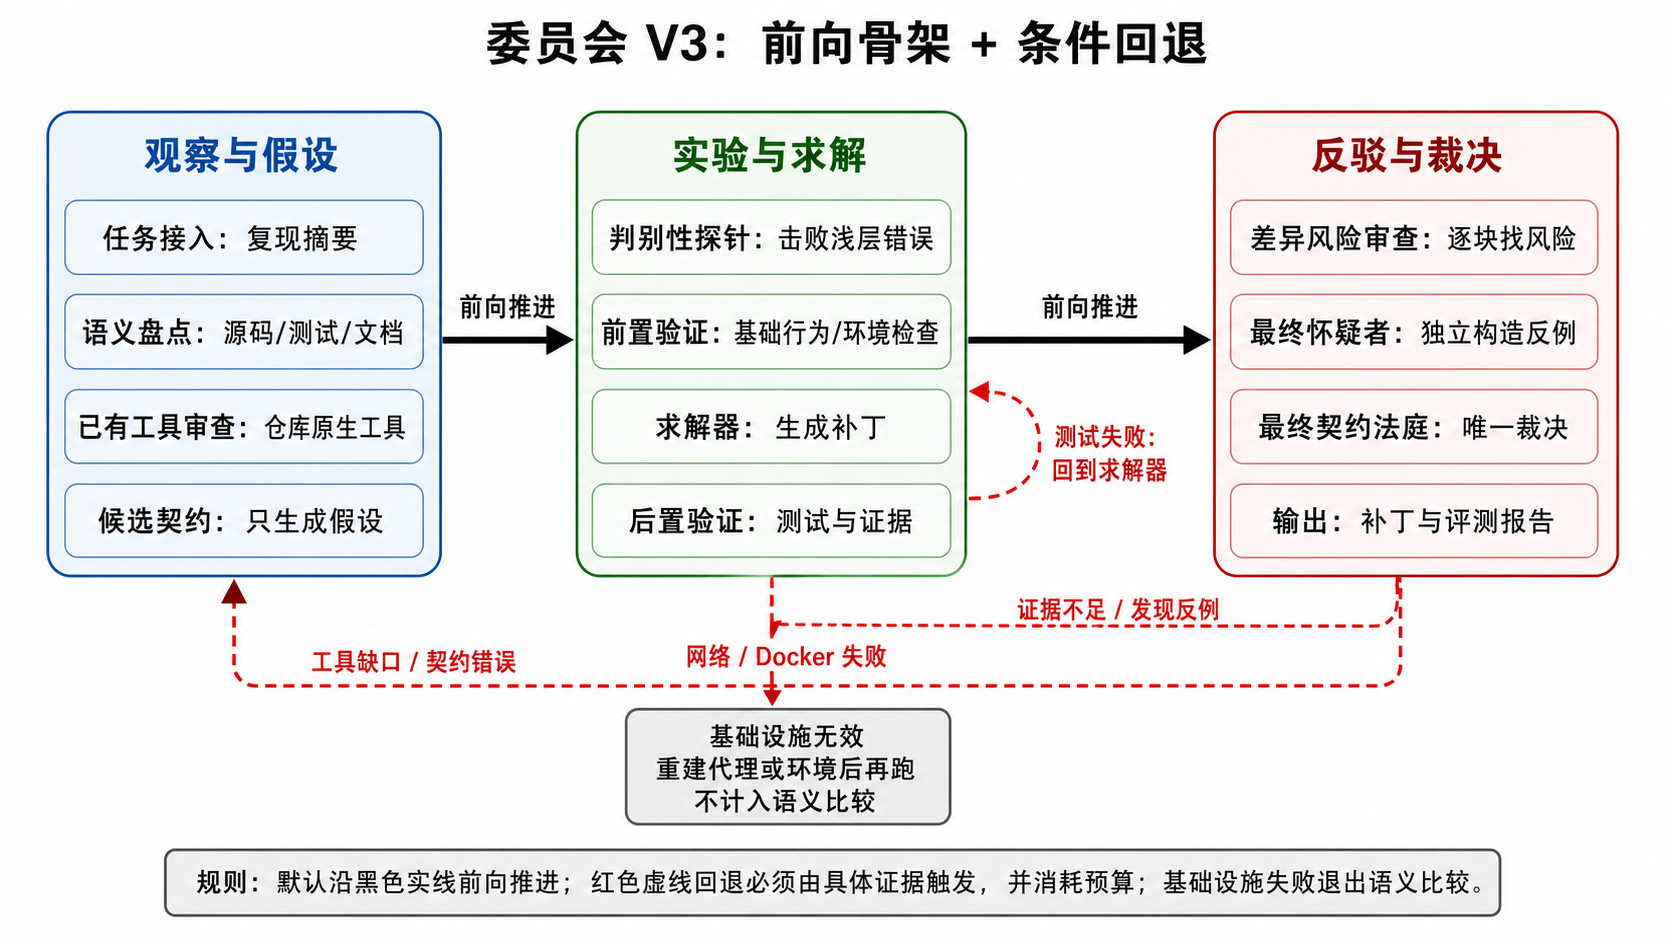
\includegraphics[width=0.98\linewidth]{v3_forward_backtrack_imagegen.png}
\caption{委员会 V3 的前向骨架与条件回退。黑色实线表示默认推进，红色虚线表示由证据触发的局部回退。}
\end{figure}

V3 的消息流使用几个固定产物。任务接入阶段产出“任务框架”，只描述问题、复现方式、相关路径和不确定点。语义盘点阶段产出“语义盘点表”，记录现有行为、测试、文档、警告文本、异常文本和公开接口兼容边界。已有工具审查阶段产出“工具审查表”，列出仓库里可复用的排序、解析、调度、图算法、序列合并等工具，并说明复用优先级。候选契约阶段产出“候选契约表”，每条契约必须标注证据等级：硬契约、有证据的假设或未知项。探针阶段产出“判别性探针包”，其中至少包含能击败浅层错误解法的探针。求解阶段产出“补丁计划”和补丁文本。验证阶段产出“验证报告”。最终契约法庭只读取这些产物，并输出“最终裁决”。括号中的英文名只作为后续实现字段名，报告叙述以中文语义为准。

\begin{table}[h]
\centering
\begin{tabularx}{0.96\linewidth}{L{3.5cm}Y Y}
\toprule
产物 & 必填内容 & 禁止内容 \\
\midrule
任务框架（\code{TaskFrame}） & 问题目标、复现线索、相关文件、未确认点 & 直接给出补丁结论 \\
语义盘点表（\code{SemanticInventory}） & 现有行为、公开测试、文档/公开接口、警告/异常精确文本 & 把题面推断写成硬契约 \\
工具审查表（\code{HelperAudit}） & 相关仓库原生工具、调用方式、复用风险、手写风险 & 在未搜索工具时接受手写通用算法 \\
候选契约表（\code{ContractHypotheses}） & 硬契约、有证据的假设、未知项、证据路径 & 早期通过/失败裁决 \\
判别性探针包（\code{ProbePack}） & 判别性探针、原始代码/补丁后的期望、命令、区分目标 & 只重复题面复现的弱探针 \\
验证报告（\code{ValidationReport}） & 测试命令、关键输出摘要、通过/失败分类 & 没有命令证据的口头确认 \\
最终裁决（\code{FinalVerdict}） & 通过/重试/基础设施无效、证据充分性、剩余风险 & 无视未知项或工具缺口直接放行 \\
\bottomrule
\end{tabularx}
\end{table}

\subsection{各委员会的权力边界}

V3 中最重要的约束是权力边界。早期的语义盘点委员会、已有工具审查委员会和候选契约委员会只能提出事实、假设和未知项。它们不能放行补丁，也不能把模型自己的推断直接升级成硬契约。判别性探针委员会负责把假设转化为可执行检查，它必须主动寻找能推翻错误实现的反例。最终契约法庭是唯一拥有“通过”权限的委员会，但它必须引用前面所有产物中的证据。

\begin{longtable}{L{3.4cm}L{4.0cm}L{7.2cm}}
\toprule
委员会 & 权限 & 失败时动作 \\
\midrule
任务接入委员会 & 设定任务边界，收集题面和复现信息 & 信息不足时返回语义盘点，不进入求解 \\
语义盘点委员会 & 读取相关源码、测试和文档，产出现有行为事实 & 未知项过多时要求继续读代码 \\
已有工具审查委员会 & 搜索仓库原生工具，判断是否应复用 & 发现未审查手写算法时阻止进入最终裁决 \\
候选契约委员会 & 把事实转成硬契约、假设、未知项三类契约 & 只能要求探针，不能裁决通过 \\
判别性探针委员会 & 设计能区分浅层错误解法的探针 & 弱探针会被最终契约法庭退回 \\
前置验证委员会 & 在原始代码或临时补丁上运行可行检查 & 环境错误归为基础设施错误，语义失败回到探针 \\
求解委员会 & 基于已知契约和工具审查表生成补丁 & 补丁触碰越界路径时退回 \\
差异风险委员会 & 按补丁差异识别新增风险和需要补测点 & 风险未覆盖时回到探针 \\
最终怀疑者委员会 & 独立构造反例，攻击补丁和验证证据 & 找到反例时回到求解或已有工具审查 \\
最终契约法庭 & 后置裁决通过、重试、基础设施无效 & 证据不足时只能重试，不能通过 \\
\bottomrule
\end{longtable}

\subsection{Prompt、结构化 I/O 与通信协议}

用人话说，V3 的做法是让一组角色接力，避免把整道题交给一个模型从头到尾自由发挥。每个角色都拿到前面角色留下的“纸条”，只能做自己那一段事，然后必须按固定格式交出下一张纸条。真实发给模型的内容由几块拼起来：全局提示词 \path{V3_WORKFLOW_AGENT_PROMPT} 先规定“谁能改代码、谁只能读和审查”；每个角色再有自己的 prompt；所有角色都拼入 \path{SHARED_RULES}，防止用隐藏测试、未来提交或把临时文件混进最终补丁；最后再拼入当前题目和前面已经产出的结构化结果。schema 的作用就是强迫模型把输出写成固定字段，后面的角色才能稳定读取。

整套通信像一场有记录的会诊。任务接入先把题目整理成任务卡；语义盘点把仓库里真实存在的行为、测试和文档列出来；已有工具审查专门找仓库里有没有现成工具；候选契约把前面看到的事实分成硬约束、合理假设和未知项；判别性探针围绕这些未知项设计能打穿错误解法的小检查；前置验证先筛掉弱检查，再跑一部分便宜检查。之后求解器才开始改代码。补丁出来以后，现有测试与批准验证会跑公开检查，差异风险审查会看补丁可能引入什么新问题，后置验证会再设计补丁后的检查，最终怀疑者会专门找反例，最终契约法庭再决定这轮能不能过。

任务接入 agent 对应 \path{V3_TASK_INTAKE_PROMPT}，label 是 \path{v3-task-intake}。它拿到的是题目 \code{goal} 和公共规则，能用的工具只有读文件和搜索。它要交出的东西叫 \code{TaskFrame}，字段包括 \code{issue_goal}、\code{reproduction_clues}、\code{related_paths}、\code{missing_information}、\code{files_to_read_next}。换句话说，它只负责把“这题到底要修什么、可能该看哪些文件、现在还缺什么信息”写清楚。它不能写补丁，也不能说补丁能过。

语义盘点 agent 对应 \path{V3_SEMANTIC_INVENTORY_PROMPT}，label 是 \path{v3-semantic-inventory}。它拿到题目和任务卡，继续读源码、公开测试、文档、警告文本、异常文本和公开 API。它交出 \code{SemanticInventory}，字段包括 \code{behavior_facts}、\code{evidence_paths}、\code{public_test_coverage}、\code{compatibility_boundaries}、\code{unknowns}、\code{risk_categories}。人话就是：它要把“仓库事实”和“题面猜测”分开。比如排序、合并、解析、调度、图算法这类容易暗藏契约的地方，它要主动标出来。

已有工具审查 agent 对应 \path{V3_HELPER_AUDIT_PROMPT}，label 是 \path{v3-helper-audit}。它拿到题目、任务卡和语义盘点，专门搜索仓库里有没有能复用的原生工具。它交出 \code{HelperAudit}，里面有 \code{search_queries}、\code{reusable_tools}、\code{reuse_priority}、\code{handrolled_risks}、\code{tool_audit_blocker}。如果任务需要写排序、解析、图算法、依赖合并这类通用逻辑，它必须先找仓库原来有没有工具。11019 就是这个点：Django 里已经有 \code{stable_topological_sort()}，所以 V3 应该先问“为什么不用这个”，再允许求解器写新算法。

候选契约 agent 对应 \path{V3_CONTRACT_HYPOTHESES_PROMPT}，label 是 \path{v3-candidate-contracts}。它拿到任务卡、语义盘点和工具审查，交出 \code{ContractHypotheses}。每条契约都有 \code{id}、\code{statement}、\code{category}、\code{evidence}、\code{validation_need}，其中 \code{category} 只能是硬约束、有证据的假设或未知项。这个角色的作用是把“我们到底相信什么”写成清单。源码、公开测试和文档支持的内容可以成为硬约束；题面例子和合理推断只能先当假设；没人能确认的东西必须交给后面的探针去验证。

判别性探针 agent 对应 \path{V3_DISCRIMINATING_PROBE_PROMPT}，label 是 \path{v3-discriminating-probes}。它拿到候选契约和工具审查，交出候选 probe。每个 probe 要写 \code{id}、关联契约、检查类型、准备方式、断言、原始代码预期、补丁后预期、它能击败哪类错误补丁、证据来源、运行命令和误报风险。人话就是：它不能只写“复现题目失败”这种浅检查，它至少要设计一个能区分“看似修了”和“真的符合仓库语义”的检查。比如 11019 里，强探针应该能打穿错误的手写拓扑排序。

前置验证由两个角色完成。先是 judge，用 \path{BASELINE_JUDGE_PROMPT} 筛掉弱 probe；再是 triage，用 \path{BASELINE_TRIAGE_PROMPT} 尝试跑一部分便宜检查。triage 的输出字段包括 \code{classifications}、\code{approved_brief}、\code{abstained}，每个检查会被标成 \code{base-fail}、\code{base-pass}、\code{invalid}、\code{weak} 或 \code{not_run} 之类。人话就是：先别急着写代码，先确认这个检查有没有意义、原始代码到底会不会暴露问题、环境有没有坏。

求解器 agent 对应 \path{V3_CODER_PROMPT}，第一轮 label 是 \path{coder:r1}，后续重试是 \path{coder-minimal-retry:rN}。它是 V3 里真正能改源码的角色，工具包含读文件、写文件、应用 patch、受限运行测试和搜索。它拿到任务卡、候选契约、工具审查、前置验证和上一轮反馈。它要做的事情很简单：在这些证据允许的范围内写最小补丁，优先复用仓库原生工具。如果它想手写通用算法，就必须解释为什么工具审查里找到的原生工具不能用。

现有测试与批准验证 agent 对应 \path{ETV_PROMPT}，label 是 \path{existing-tests-approved-validation:rN}。它拿到 coder 的说明、前置 judge 和 triage 结果，负责跑公开测试和已批准的验证检查，并记录补丁边界。它输出 \code{status}、\code{findings}、\code{checks}、\code{allowed_patch_paths}、\code{disallowed_patch_paths}。人话就是：它检查“补丁有没有跑过该跑的公开测试、有没有把临时文件或测试文件混进最终 diff、哪些文件改动是允许的”。

三路差异风险 agent 是补丁出来后的三种挑刺方式。 \path{branch-boundary-attack:rN} 找边界和分支风险，\path{regression-scan:rN} 找相邻行为回归，\path{observable-diff-review:rN} 读当前 diff，看有没有缺少契约支持的可观察变化。三者都输出风险清单，每个风险包含位置、风险描述、关联契约、建议补测和优先级。代码会把三路结果合并成 \code{diff_risks}，交给后置验证和最终法庭。

后置验证工厂对应 \path{V3_POST_VALIDATION_FACTORY_PROMPT}，label 是 \path{post-validation-factory:rN}。它拿到候选契约和差异风险，继续设计补丁后的 probe。随后 post judge 用 \path{POST_JUDGE_TRIAGE_PROMPT} 运行这些 probe，并输出 \code{verdict}、\code{accepted}、\code{rejected}、\code{diagnostic}、\code{triage}、\code{validation_brief}、\code{retry_feedback}。这里最关键的规则是：只有接受的、有证据支持的检查明确失败时，才返回 \code{FAIL_WITH_EVIDENCE}，然后直接把问题交回求解器重试。弱检查、诊断检查、没跑起来的检查不能把补丁判死。

最终怀疑者 agent 对应 \path{V3_FINAL_SKEPTIC_PROMPT}，label 是 \path{final-skeptic:rN}。它拿到任务卡、候选契约、验证结果、差异风险和后置验证结果，专门站在反方找最小反例。它输出 \code{verdict}、\code{findings}、\code{required_evidence}、\code{next_action}。如果它认为问题来自契约证据不足，就给出 \code{CONTRACT_EVIDENCE_BLOCKER}，代码会回到候选契约重新仲裁，再重新做探针。人话就是：它负责防止大家拿着一套不够硬的契约往后走。

最终契约法庭 agent 对应 \path{V3_FINAL_TRIBUNAL_PROMPT}，label 是 \path{final-contract-tribunal:rN}。它拿到前面所有材料，输出 \code{PASS} 或 \code{CONCRETE_BLOCKER}。它的结构化输出里必须有 \code{verification_coverage}，里面要写判别性探针、仓库原生工具复用审查、API 兼容检查、新证据摘要和覆盖缺口。人话就是：最终法庭只问一件事，当前补丁的证据够不够交卷。证据够才通过；证据缺了，就把缺什么说清楚，交给下一轮求解器。

输出节点没有 LLM prompt。只有最终契约法庭返回 \code{PASS}，\path{swe_committee_v3()} 才返回 \code{status=done}，并带上任务卡、语义盘点、工具审查、候选契约、probe 数量、验证覆盖、每轮尝试、token 和失败计数。外层脚本再抽取 staged diff 写入 \path{predictions.jsonl}，然后做题脚本把非空 patch 送去 official eval。

这套实现已经把“谁负责观察、谁负责改代码、谁负责验证、谁负责否决”分清楚了，但真实核心 prompt 仍然偏短。最需要继续加厚的是判别性探针、后置验证工厂和最终怀疑者：它们应该有更多强探针例子、弱探针反例、手写算法攻击模板和明确回退规则。否则委员会看起来很完整，实际还是可能放过一个浅层错误补丁。

\subsection{V3 对 11019 的预期行为}

在 \code{django__django-11019} 上，V3 应该在求解前发现两个关键事实。语义盘点委员会会把 \code{Media.merge()} 的稳定交错顺序列为高风险契约；已有工具审查委员会会发现 Django 已有的稳定拓扑排序工具 \code{stable_topological_sort()}，并要求优先复用。候选契约委员会只能把题面复现转为有证据的假设，不能直接裁决手写拓扑排序可行。判别性探针委员会必须生成“输入 \code{[1,2]} 与 \code{[3,4]} 应得到 \code{[1,3,2,4]}”这类探针。最终法庭看到手写算法没有通过稳定交错探针或没有解释工具审查结果时，应返回“重试”，拒绝接受该补丁。

这个设计的实验目标很明确。第一，V3 应使 \code{django__django-11019} 从稳定错误手写算法转向复用 \code{stable_topological_sort()} 或等价正确实现。第二，V3 应保持 \code{django__django-14730} 通过。第三，V3 在连接错误冒烟样本上应继续把基础设施失败排除出语义比较。第四，V3 的令牌成本要和 V2 对比，如果 V3 只增加成本但没有提升工作流完整完成率和官方通过率，就需要继续做消融。

\section{自动做题脚本}

生成 patch 和评测 patch 已合并为“做题”。新增脚本 \code{scripts/swe_auto_eval_driver.py} 是这套流程的中心。它从远端 \code{predictions.jsonl} 发现非空 patch，按 \code{instance id + patch sha} 生成稳定候选，创建 side-car 输入文件，启动 official eval tmux，并把状态写回远端与本地监控文件。它不调用模型，也不读取 API key。

脚本已经处理以下实际问题。tmux 已经退出时，状态会从 active 刷新为 pending、done 或失败状态。report discovery 会同时检查 side-car 根目录、official eval 目录和 \code{/home/dongyh}，避免已完成评测被误判为 missing report。SSH 断连会写 \code{ssh_error} 快照并在 watch 模式继续下一轮。side-car 加了互斥锁，减少两个 driver 同时启动同一 patch 的风险。dataset 输入会把单对象 JSON 规范成单元素 list，并校验其中包含当前题目的 \code{instance_id}。输出路径会进行 token/key redaction 检查。

当前自动做题脚本在 \code{django__django-11019} 上的真实验证结果为：1 个 prediction row，1 个 patch 已 official eval，resolved 为 0，unresolved 为 1，active generation 和 active eval 会话均为空。对应监控文件为 \path{docs/monitoring/swe_auto_eval_status.md} 与 \path{docs/monitoring/swe_auto_eval_status.json}。

\section{做题 Skill}

为了让后续任务自动触发统一流程，已创建用户级 skill：

\path{/Users/Kai/.codex/skills/swebench-do-task/SKILL.md}

它的触发词覆盖“做题”“跑题”“生成 patch”“评测 patch”“SWE-bench”“V1/V2 对比”“official eval”等表达。skill 中明确规定，做题优先由脚本驱动；遇到可复现的小问题时先改脚本，再继续执行。这样后续同类工作会积累到同一个 harness 中，减少重复人工判断。

\section{下一步实验设计}

下一轮实验应先小规模验证，再扩展到更大的消融比较。短期应继续用 \code{django__django-11019} 检查判别性探针和“已有工具优先”审查是否能修复 V2 回归，同时保持 \code{django__django-14730} 作为正向样本。Connection-error smoke 样本仍然适合做基础设施稳定性检查，例如 \code{astropy__astropy-7746}、\code{django__django-11905} 和 \code{django__django-14155}。

消融比较建议包含 V1、V1 加 observable inventory、V1 加三路 diff-risk、V1 加 final skeptic、完整 V2。每个条件记录 resolved、F2P fail、P2P fail、patch rate、workflow done rate、infra invalid rate、input/output/cached token，以及内部 verdict 与官方评测的一致性。

\section{证据路径}

\begin{longtable}{L{5.2cm}L{9.9cm}}
\toprule
用途 & 路径 \\
\midrule
V2 11 题监控 Markdown & \path{docs/monitoring/swe_v2_11_status.md} \\
V2 11 题监控 JSON & \path{docs/monitoring/swe_v2_11_status.json} \\
11019 V1/V2 分析 & \path{docs/monitoring/swe_v2_11019_v1_v2_regression_analysis.md} \\
自动做题状态 Markdown & \path{docs/monitoring/swe_auto_eval_status.md} \\
自动做题状态 JSON & \path{docs/monitoring/swe_auto_eval_status.json} \\
自动做题脚本 & \path{scripts/swe_auto_eval_driver.py} \\
V2 队列 driver & \path{scripts/swe_v2_queue_driver.py} \\
V2 workflow & \path{workflows/swe_committee_v2.py} \\
做题 skill & \path{/Users/Kai/.codex/skills/swebench-do-task/SKILL.md} \\
\bottomrule
\end{longtable}

\end{document}
